% отчет по практике
\documentclass[master, och, times, pract]{sty/SCWorks}

\usepackage[T2A]{fontenc}
\usepackage[utf8]{inputenc}
\usepackage{graphicx}
\usepackage{float}

\usepackage[sort,compress]{cite}
\usepackage{amsmath}
\usepackage{amssymb}
\usepackage{amsthm}
\usepackage{longtable}
\usepackage{array}
\usepackage[english,russian]{babel}
\usepackage{amsfonts}
\usepackage{commath}
\usepackage{amsthm}

\usepackage[colorlinks=true]{hyperref}

\usepackage{listings}

\usepackage[ruled,vlined,linesnumbered,resetcount,algosection]{algorithm2e}

\usepackage{algpseudocode}

\usepackage{longtable,rotating}
\usepackage{threeparttable}

% для кода
\usepackage{fancyvrb}
\DefineShortVerb{\|}

% для картинок
\usepackage{chngcntr}
\counterwithin{figure}{section}

\theoremstyle{plain}
\newtheorem{thethm}{Теорема}[section]
\newtheorem{lemma}{Лемма}[section]
\newtheorem{note}{Замечание}[section]
\newtheorem{proposition}{Предложение}[section]
\newtheorem{exmp}{Пример}[section]
\newtheorem{problem}{Проблема}[section]

\theoremstyle{definition}
\newtheorem{defn}{Определение}[section]

\numberwithin{equation}{section}

\SetKwInput{KwData}{Исходные параметры}
\SetKwInput{KwResult}{Результат}
\SetKwInput{KwIn}{Входные данные}
\SetKwInput{KwOut}{Выходные данные}
\SetKwIF{If}{ElseIf}{Else}{если}{тогда}{иначе если}{иначе}{конец условия}
\SetKwFor{While}{до тех пор, пока}{выполнять}{конец цикла}
\SetKw{KwTo}{от}
\SetKw{KwRet}{возвратить}
\SetKw{Return}{возвратить}
\SetKwBlock{Begin}{начало блока}{конец блока}
\SetKwSwitch{Switch}{Case}{Other}{Проверить значение}{и выполнить}{вариант}{в противном случае}{конец варианта}{конец проверки значений}
\SetKwFor{For}{цикл}{выполнять}{конец цикла}
\SetKwFor{ForEach}{для каждого}{выполнять}{конец цикла}
\SetKwRepeat{Repeat}{повторять}{до тех пор, пока}
\SetAlgorithmName{Алгоритм}{алгоритм}{Список алгоритмов}

\algrenewcommand\algorithmicfunction{\textbf{Функция}}
\algrenewcommand\algorithmicprocedure{\textbf{Процедура}}
\algrenewtext{EndFunction}{\textbf{Конец функции}}
\algrenewtext{EndProcedure}{\textbf{Конец процедуры}}

\begin{document}

% Кафедра (в родительном падеже)
\chair{дискретной математики}
% Тема работы
\title{}
% Курс
\course{2}
% Группа
\group{271}
% Специальность/направление код - наименование
\napravlenie{09.04.01 "--- Информатика и вычислительная техника}

\term{4}

\duration{5}
\practtype{преддипломная}

\title{}

\practStart{16.04.20}
\practFinish{27.05.20}

% Фамилия, имя, отчество в родительном падеже
\author{Шарова Александра Вадимовича}
% Заведующий кафедрой
\chtitle{к.\,ф.-м.\,н., доцент} % степень, звание
\chname{Л.\,Б.\,Тяпаев}
%Научный руководитель (для реферата преподаватель проверяющий работу)
\satitle{к.\,ф.-м.\,н., доцент} %должность, степень, звание
\saname{Л.\,Б.\,Тяпаев}
% Руководитель практики от организации (только для практики,
% для остальных типов работ не используется)
\patitle{к.\,ф.-м.\,н., доцент}
\paname{Л.\,Б.\,Тяпаев}

% Год выполнения отчета
\date{2020}

\maketitle
\tableofcontents


\intro

Цель данной практики -- разработка практической части для магистерской выпускной квалификационной работы, а именно доработка многопоточного варианта библиотеки для работы с $p$-адической арифметикой, а также доработка однопоточного варианта $p$-адической арифметики, который был представлен на студенческой научной конференции в Апреле для задачи вычисления матричной экспоненты.

В течение периода практики была доработана однопоточная библиотека для работы с $p$-адической арифметикой, реализованы новые возможности одна из которых это перегрузка операторов для класса |Padic| и |Matrix|. После этого библиотека была расширена с помощью применения параллельного программирования на многопоточный случай. Как для многопоточной, так и для однопоточной библиотеки были произведены тесты производительности, где в качестве примера использовались такие прикладные задачи как нахождение решения СЛАУ, ОДУ, вычисление собственных чисел и собственных значений векторов матрицы, вычисление матричной экспоненты. Все тесты производились с использованием чисел из таких числовых полей, как $\mathbb{Q}_2$, $\mathbb{Q}_3$, $\mathbb{Q}_5, \mathbb{Q}_5$ и $\mathbb{Q}_{23}$.

Полученные во время практики результаты были использованы в практической части магистерской выпускной квалификационной работы. 


%-------------------------------------------------------------------%
\section{Разработка однопоточной библиотеки для работы с $p$-адической арифметикой}

Библиотека для работы с $p$-адической арифметикой будет состоять из набора модулей, которые представляют из себя единый пакет для ЯП Python. Данный пакет может быть загружен как зависимость при помощи пакетного менеджера |pip| с помощью спецификации в файле |requirements.txt|, что без проблем позволяет переиспользовать разработанную библиотеку. Однопоточная библиотека будет содержать следующие модули:

\begin{itemize}
\item Модуль для работы с $p$-адическими числами. Содержит базовые арифметические и алгебраические операции, а также представляет основные программные интерфейсы, например, ввод и вывод чисел в человекочитаемом формате.
\item Модуль для работы с матрицами и векторами. Предоставляет базовые операции над матрицами, а также вспомогательные функции для выполнения математических операций с использованием матричной арифметики.
\item Модуль с реализацией таких базовых алгоритмов, как вычисление определителя матрицы, решение СЛАУ методами Крамера и Гаусса, алгоритм Якоби для вычисления собственных значений и собственных векторов. Кроме того данный модуль содержит реализацию решения дифференциальных уравнений методами Эйлера и методом Рунге-Кутта четвертого порядка.
%\item Модуль с синтетическими тестами. Будет использоваться для сравнения обычных и $p$-адических методов.
\end{itemize}

%-------------------------------------------------------------------%
\subsection{Описание типов данных}

Для описания таких типов данных, как матрицы и $p$-адические числа, был выбран объектно-ориентированный подход. Данный подход позволяет оперировать с $p$-адическими числами и матрицами аналогично тому, как это происходит в математике. Также ООП позволяет программисту не думать о том, какие методы нужны для работы с данными, которые он уже определил. Это следует из основной концепции ООП: данные всегда находятся рядом с методами, которые оперируют над ними. Стоит также добавить, что в ЯП Python распространена ООП реализация математических структур во многих популярных библиотеках, которые имеют много методов и алгоритмов для работы с данными. Данных подход является стандартом.

\subsubsection{$p$-адические числа}

Для описания $p$-адических чисел реализован Python класс |PAdic(object)|. Перед тем как переходить к описанию методов и способов инициализации класса, необходимо описать, каким образом устроен конструктор класса. На вход конструктору класса |PAdic(object)| подается либо целое число, либо строка. Строка для конструктора выбрана для того, чтобы можно было легко инициализировать объекты рациональными числами, не беспокоясь о том, что ЯП Python приведет их к действительным числам негласно, таким убирается снимается неопределенное поведение программы Стоит отметить, что строковый тип данных используется только на этапе инициализации $p$-адического числа, все дальнейшие операции внутри класса происходят с помощью числовых примитивов, представленных в ЯП Python.

Рассмотрим инициализацию объекта, который представляет собой $p$-адическое число. Данное действие можно сделать несколькими способами с использованием различных представлений, а именно:

 \begin{itemize}
 \item С помощью задания непосредственно числа и базы. Например, такое объявление создания объекта, как |p = PAdic("3/4", 5)|, -- это инициализация объекта класса |PAdic| числом \mbox{$\frac{3}{4} \in \mathbb{Q}_5$}. Стоит отметить, что поддерживаются не \mbox{только} числа из поля целых чисел $\mathbb{Z}$, но и числа из поля рациональных чисел $\mathbb{Q}$ в виде |"a/b"|. Данное действие возможно благодаря использованию представления числа в виде строки в качестве входного параметра для конструктора класса.
 \item С помощью уже известной последовательности. Например, когда мы уже знаем $p$-адическое представление числа $a$ и нам нужно создать объект, чтобы было возможно продолжить оперировать данным числом в программе. В этом случае инициализация объекта будет выглядеть следующим образом: |PAdic({[4,0,0,0], 3, False}, 2, 'SEQUENCE')|.
 \end{itemize}

Стоит отметить, что в ЯП Python невозможно реализовать перегрузку конструкторов, и по этой причине конструктор является достаточно комплексным. Данное явление является нормой для всех математических пакетов, представленных для ЯП Python, и продиктовано ограничениями языка.


Перейдем к рассмотрению основных особенностей типа данных для работы с $p$-адическими числами:

\begin{itemize}

\item Вычисления, производимые в поле $\mathbb{Q}$, не накапливают ошибку с увеличением числа операций. Каждое рациональное число представляется в качестве конечной последовательности целых чисел и при увеличении числа операций арифметическая ошибка не накапливается\cite{bib:computation:gregory}.

\item Целочисленные вычисления происходят с максимально возможным использованием классической архитектуры компьютера. Обычно вычисления, оперирующие с рациональными числами, используют представление числа в виде числителя и знаменателя. Допустим, что каждая цифра числа будет занимать $1$ байт. Тогда при выполнении следующего сложениния:

$$
\begin{tabular}{ccccccccccc}
& + & 1 & 2\; & 3\; & 4\; & 5\; & 6 & 7\; &  \\
& = & 7 & 6\; & 5\; & 4\; & 3\; & 2\; & 1\; &  \\
\hline
& = & 8\; & 8\; & 8\; & 8\; & 8\; & 8\; & 8\; &
\end{tabular}
$$

будет произведено 16 операций с символами. Если взять $p$-адический тип данных, где $p=46337$, то количество операций можно сильно сократить:

$$
\begin{tabular}{ccccccccccc}
& + & 29805 & 25\; & 0\; &  \\
& = & 8716 & 165\; & 0\; & \\
\hline
& = & 38521\; & 191\; & 0\; &
\end{tabular}.
$$

В данном случае будут произведены только $3$ операции сложения и $3$ операции сравнения по модулю.

\item Параллельная структура, которая позволяет полноценно и равномерно использовать многоядерную систему. Вне зависимости от алгоритма, работающего с базовыми арифметическими операциями, будет использоваться параллельная реализация алгоритма работы с базовой арифметикой.
\item Структура данных, готовая для равномерного распределения задач в облачной среде. При операциях представленным типом данных общая нагрузка на центральный процессор может равномерно распределяется на мелкие части. Кроме того, в рациональной арифметике такой процесс, как вычисление числа, сильно увеличивает потребление памяти, в то время как в $p$-адическом типе данных такой проблемы нет. Количество памяти не будет расти в процессе работы, потому память для $p$-адического типа данных выделяется всего один раз при создании объекта класса. Благодаря этому легко рассчитать приблизительное количество потребляемой памяти перед запуском программы в случае необходимости.
\item cloud-ready тип данных. При использовании данного типа его модули имеют слабую связность. Исходя из этого каждый модуль может быть рассчитан параллельно на различных узлах кластера или на различных машинах в облаке.
\end{itemize}

Перейдем к рассмотрению основных методов класса |PAdic|. Данные методы реализуют базовые математические операции с $p$-адическими числами, представленными в виде кода Гензеля:

\begin{itemize}
\item Сложение $p$-адических чисел. Данная операция реализована с помощью метода |__add__|, этот метод является одним из многих так называемых |Magic Methods|, которые позволяют делать перегрузку операторов в ЯП Python и предоставляют пользователю возможность работы с математическими объектами более естественным образом, а именно с помощью использования знака |"+"| в программе вместо явного вызова функции, имя которой пользователю может быть неизвестно без подробного ознакомления с документацией и исходным кодом библиотеки. Сам метод |__add__| является в свою очередь оберткой над методом |add_by_offset|, который представляет собой сложение $p$-адических чисел, представленных в виде кода Гензеля.
\item Вычитание $p$-адических чисел. Данный метод реализован аналогично сложению за исключением того, что использует метод |__sub__|, позволяющий использовать в коде знак |"-"| при работе с $p$-адическими числами естественным образом. Метод по аналогии со сложением является оберткой над методом |subtract_by_offset|, который тоже оперирует с числами, представленными в виде кода Гензеля.
\item Вычисление числа со знаком минус. Данная операция реализована с помощью метода |__neg__|. В коде это может быть использовано как |a = -b|, где |b| -- это произвольное $p$-адическое число.
\item Вычисление числа со знаком плюс. Данная операция реализована с помощью метода |__pos__|. В коде это может быть использовано как |a = +b|, где |b| -- это произвольное $p$-адическое число. Данная унарная операция обычно реализуется в классах для симметрии. Так как унарный минус является оператором, унарный плюс тоже должен быть представлен в качестве оператора.
\item Умножение $p$-адического числа на целое число из поля $\mathbb{Z}$. Данную операцию реализует метод |multiply_to_integer|, который производит умножение $p$-адического числа на целое число, представленное элементарным типом данных ЯП Python.
\item Умножение $p$-адических чисел. Данная операция реализована с помощью метода |__mul__|, который нужен для возможности использования знака |"*"| при работе с числами и представляет собой метод, реализующий $p$-адическое умножение чисел, представленных кодом Гензеля.
\item Деление $p$-адических чисел. Данная операция реализована с помощью метода |__truediv__|, который нужен для возможности использования знака |"/"| при работе с числами и представляет собой метод реализующий $p$-адическое умножение чисел, представленных кодом Гензеля.
\item Вычисления порядка $p$-адического числа. Операция реализована методом |calculate_order|. Метод является статическим, а значит, может быть вызван для любого объекта класса извне с помощью вызова метода |PAdic.calculate_order(a)|, где |a| -- это некоторое $p$-адическое число.
\item Получение порядка $p$-адического числа. Операция реализована методом |get_order| и возвращает порядок $p$-адического числа в виде числа, представленного элементарным типом данных.
\item Вывод $p$-адического числа в человекочитаемом формате. Данная возможность реализована  помощью метода |__str__|. Поскольку встроенная в ЯП Python функция |print()| использует именно функцию |str()| для вывода объекта любого класса на экран, то определение метода |__str_| позволит выводить объекты на экран стандартным способом при помощи встроенной функции  |print()|.
\item Вывод $p$-адического числа в виде объекта класса |PAdic(object)|. Данная возможность реализована с помощью метода |__repr__| возвращающего строку с описанием объекта, который может быть воспринят итерпретатором ЯП Python без изменений. Это значит, что вывод может быть скопирован в программу без изменений и будет представлять собой корректный код.
%\item find_multiplier
%\item do_eratosthene_sieve
%\item check_for_base_equality
%\item check_for_prime
\end{itemize}

Стоит отметить, что для типа данных, который работает с $p$-адической арифметикой, очень важно выбрать правильный набор простых чисел $\{ p_1, p_2, \cdots, p_s \}$. Согласно теории, чем больше выбор числа $s$, тем больше будет верхняя граница возможных вычислений. Когда мы используем целочисленную арифметику для компьютеров с 32-х или 64-х битной архитектурой, наибольший $p_i$ должен быть либо  $46337$, либо  $2147483647$, чтобы избежать переполнения. Это значит, что для 32-х битной архитектуры $p_i \leq 46337$, тогда как для 64-х битной архитектуры $p_i \leq 2147483647$. Данные ограничения являются фундаментальными для $p$-адического типа данных, но ими можно пренебречь при использовании символьной арифметики.


\subsubsection{Матрицы и вектора}

Для работы с матрицами и векторами реализован Python класс |Matrix(object)|, который позволяет работать не только с обыкновенными типами чисел (как, например, в пакете |numpy|), но и с $p$-адическими числами. Данный класс содержит следующие методы:

\begin{itemize}
\item Метод |__getitem__| позволяет получать элементы матрицы с помощью стандартной операции взятия индекса, а именно |A[i][j]|. Данная операция очень важна, так как в алгоритмах работы с матрицами почти всегда нужно оперировать элементами при помощи индексов.
\item Метод |__setitem__| позволяет устанавливать элементы матрицы с помощью стандартной операции работы с индексами, а именно |A[i][j]=2|. Аналогично методу |__getitem__| данная операция является основополагающей.
\item Метод |get_rank|. Реализует возможность вычисления ранга матрицы -- наивысшего из порядков всевозможных ненулевых миноров матрицы.
\item Метод |reset| -- очистка матрицы для дальнейшего переиспользования уже существующего объекта. Данный метод нужен нечасто, но иногда бывает очень удобен, например, при обнулении матрицы в зависимости от конкретных условий в ряде алгоритмов
\item Метод |transpose| -- транспонирование матрицы. Возвращает $A^{T}$, полученную из исходной матрицы $A$ путем замены строк на столбцы. Оперирует с текущем обьектом.
\item Метод |get_transpose| -- получение транспонированной матрицы $A^{T}$ в виде нового объекта на основании уже существующего объекта.
\item Метод |__add__| реализует возможность складывать матрицы с помощью бинарного оператора |"+"|.
\item Метод |__iadd__| определяет возможность присвоения со сложением с помощью оператора |"+="|. Данный метод позволяет использовать конструкцию |A += B| вместо конструкции |A = A + B|.
\item Метод |__sub__| реализует возможность вычитать матрицы с помощью бинарного оператора |"-"|.
\item Метод |__isub__| определяет возможность присвоения с вычитанием с помощью оператора |"-="|. Данный метод позволяет использовать конструкцию |A -= B| вместо |A = A - B|.
\item Метод |__mul__| определяет возможность умножать матрицы с помощью бинарного оператора |"*"|.
\item Метод |__imul__| определяет возможность присвоения с умножением с помощью оператора |"*="|. Данный метод позволяет использовать конструкцию |A *= B| вместо |A = A * B|.
\item Метод |__eq__| реализует возможность сравнения двух матриц с помощью стандартного оператора |"="|.
\item Статический метод |make_matrix| заполняет объект массивом строк, поданным на вход.
\item Статический метод |make_random| возвращает матрицу со случайными значениями элементов.
\item Статический метод |make_zero| возвращает матрицу, заполненную нулевыми значениями.
\item Статический метод |make_id| возвращает единичную матрицу $E$, элементы главной диагонали которой равны единице поля, а остальные равны нулю.
\item Вывод матрицы в человекочитаемом формате. Данная возможность реализована с помощью метода |__str__|. Поскольку функция |print| использует именно функцию |str()| для вывода объекта на экран, то определение метода |__str__| позволит выводить объекты на экран стандартным способом при помощи встроенной функции |print()|.
\item Вывод матрицы в виде объекта класса |Matrix|, который может быть корректно воспринят интерпретатором ЯП Python. Данная возможность реализована с помощью метода |__repr__|, который возвращает строку с описанием объекта в виде Python кода.
\end{itemize}


\subsection{Примеры использования библиотеки}

Так как библиотека основана на объектно-оринтированном подходе и практически все математические операторы перегружены как для матриц, так и для $p$-адических чисел, то использование базовых математических операций является достаточно естественным процессом для программиста.

\begin{exmp}
Сложить числа $\frac{3}{2}$ и $\frac{1}{2}$ в $\mathbb{Q}_5$ и вывести представление полученной суммы на экран.
\begin{lstlisting}[language=Python, numbers=left, showstringspaces=false, breaklines=true, basicstyle=\small]
from padic.padic import *
print(PAdic("3/2", 5) + PAdic("1/2", 5))
\end{lstlisting}

\noindent Выводом для данной программы будет число $2 \in \mathbb{Q}$.
\end{exmp}

\begin{exmp}
Найти разность чисел $\frac{3}{4}$ и $\frac{3}{2}$ в $\mathbb{Q}_5$ и вывести представление полученной разности на экран.
\begin{lstlisting}[language=Python, numbers=left, showstringspaces=false, breaklines=true, basicstyle=\small]
from padic.padic import *
print(PAdic("3/4", 5) - PAdic("3/2", 5))
\end{lstlisting}

\noindent Выводом для данной программы будет число $.33333\dots \in \mathbb{Q}_5$.
\end{exmp}


\begin{exmp}
Умножить число $\frac{1}{13}$ на число $13$ в $\mathbb{Q}_{101}$ и вывести результат на экран.
\begin{lstlisting}[language=Python, numbers=left, showstringspaces=false, breaklines=true, basicstyle=\small]
from padic.padic import *
print(PAdic("1/13", 101) + PAdic("13", 101))
\end{lstlisting}

\noindent Выводом для данной программы будет число $1 \in \mathbb{Q}$.
\end{exmp}


\begin{exmp}
Разделить число $3$ на число $\frac{1}{3}$ в $\mathbb{Q}_{167}$ и вывести результат на экран.
\begin{lstlisting}[language=Python, numbers=left, showstringspaces=false, breaklines=true, basicstyle=\small]
from padic.padic import *
print(PAdic("3", 167) + PAdic("1/3", 167))
\end{lstlisting}

\noindent Выводом для данной программы будет число $9 \in \mathbb{Q}$.
\end{exmp}


\begin{exmp}
Вычислить определитель матрицы

$$
\begin{pmatrix}
  1 & 4 \\
  0 & 3
\end{pmatrix}.
$$

\begin{lstlisting}[language=Python, numbers=left, showstringspaces=false, breaklines=true, basicstyle=\small]
from padic.padic import *
from padic.matrix import *
m = Matrix(2, 2)
m1[0] = [PAdic("1", 7),PAdic("4", 7)]
m1[1] = [PAdic("0", 7),PAdic("3", 7)]
print(Matrix.det())
\end{lstlisting}

\noindent Выводом для данной программы будет число $3 \in \mathbb{Q}$.
\end{exmp}

\begin{exmp}
Решить СЛАУ методом Крамера

$$
\begin{cases}
  2x_1 + x_2 + x_3 = 2 \\
  x_1 - x_2 = -2 \\
  3x_1 - x_2 +2x_3 =2
\end{cases}.
$$

\begin{lstlisting}[language=Python, numbers=left, showstringspaces=false, breaklines=true, basicstyle=\small]
from padic.padic import *
from padic.matrix import *
from algo import *
dim = 3
A = Matrix(dim, dim)
A[0] = [PAdic("2", 5), PAdic("1", 5), PAdic("1", 5)]
A[1] = [PAdic("1", 5), PAdic("-1", 5), PAdic("0", 5)]
A[2] = [PAdic("3", 5), PAdic("-1", 5), PAdic("2", 5)]
B = [PAdic("2", 5), PAdic("3", 5), PAdic("3", 5)]
X = cramer(A, B)
print(X)
\end{lstlisting}

\noindent Выводом для данной программы будет вектор $[.44444, 1, 3]$, где число $(.4444)_5 \in \mathbb{Q}_5$ представляет собой число $-1 \in \mathbb{Q}$. Видно, что два числа выведены в $\mathbb{Q}$, а одно в $\mathbb{Q}_5$. Это нормальное поведение, так как библиотека старается использовать обыкновенные рациональные числа в качестве выходных значений. Для того чтобы определить однозначный формат выходных данных, в программе данная функция может быть отключена. В этом случае в качестве выходных данных всегда будут использоваться только $p$-адические числа.
\end{exmp}

\begin{exmp}
Решить СЛАУ методом Гаусса

$$
\begin{cases}
  3x_1 - 2x_2 = -6 \\
  5x_1 + x_2 = 3
\end{cases}.
$$

\begin{lstlisting}[language=Python, numbers=left, showstringspaces=false, breaklines=true, basicstyle=\small]
from padic.padic import *
from padic.matrix import *
from algo import *
dim = 2
A = Matrix(dim, dim)
A[0] = [PAdic("3", 5), PAdic("-2", 5)]
A[1] = [PAdic("5", 5), PAdic("1", 5)]
B = [PAdic("-6", 5), PAdic("3", 5)]
X = gauss(A, B)
print(X)
\end{lstlisting}

\noindent Выводом для данной программы будет вектор $[0, 3]$. Оба значения вектора решения выведены в виде обычных рациональных чисел.
\end{exmp}


\subsection{Сравнение производительности классических и $p$-адических \mbox{методов}}

\subsubsection{Вычисление определителя матрицы}

Для сравнения производительности классического и $p$-адического метода вычисления определителя матрицы вычислим определитель для случайно сгенерированной матрицы $\boldsymbol{A}$, у которой коэффициенты вычисляются следующим образом:
\begin{equation}
a_{i,j}=
\begin{cases}
1-\bigg(round\bigg(\frac{i-j}{n}\bigg)\bigg)^2, \; i \neq j, \\
10-round\bigg(\frac{i-j}{n}\bigg), \; i = j.
\end{cases}
\end{equation}

Производительность методов вычисления определителя будем \mbox{тестировать} на матрице, размер которой равен $1000 \times 1000$. Вычисление будем повторять $100$ раз. Время решения будем измерять по циклу вычисления определителя без учета предварительной подготовки \mbox{матрицы $\boldsymbol{A}$}.

Разные запуски реализаций решения на ПК дают несколько разное время, поскольку ОС периодически отбирает ресурсы от запущенной программы для своих нужд. Из нескольких запусков будем записывать минимальное время.

Также для наглядности будем сравнивать различные числа из таких полей, как $\mathbb{Q}_2$, $\mathbb{Q}_3$, $\mathbb{Q}_5$, $\mathbb{Q}_7, \mathbb{Q}_{23}$.

\begin{figure}[H]
\centerline{\includegraphics[width=0.85\linewidth]{../gnuplot/single/det/plot.png}}
\caption{График производительности однопоточных методов для вычисления определителя матрицы.}
\label{img:single:det:1}
\end{figure}

\begin{figure}[H]
\centerline{\includegraphics[width=0.85\linewidth]{../gnuplot/single/det/wosymb.png}}
\caption{График производительности однопоточных методов для вычисления определителя матрицы (без символьного метода).}
\label{img:single:det:2}
\end{figure}

Как видно из результатов, обычные методы из пакета |numpy| работают немного быстрее, чем $p$-адические методы, а методы из пакета |scipy| работают сопоставимое с $p$-адическими методами время. На графике \ref{img:single:det:2} видно, что символьные методы работают в разы дольше, чем классические и $p$-адические методы.

\subsubsection{Решение СЛАУ}
Для сравнения производительности классического и $p$-адического метода решения СЛАУ решим $m$ раз систему из $n$ уравнений:

\begin{equation}
\boldsymbol{A}*\boldsymbol{X}=\boldsymbol{B},
\end{equation}

\noindent где $\boldsymbol{A}$ - матрица коэффициентов размером $n \times n$, $\boldsymbol{X}$ - вектор неизвестных и $\boldsymbol{B}$ - вектор правых частей.
Пусть коэффициенты матрицы $\boldsymbol{A}$ вычисляются следующим образом:

\begin{equation}
a_{i,j}=
\begin{cases}
\abs{1-rand(n)*round\bigg(i-j\bigg)^2}, i \neq j, \\
10, i = j,
\end{cases}
\end{equation}

\noindent где |rand(n)| -- некоторое случайное число в диапазоне от $0$ до $n$. При этом получается положительно определенная матрица. Например, для $n=5$ матрица $\boldsymbol{A}$ будет иметь вид:

$$
\begin{pmatrix}
  10 & 7 & 23 & 53 & 79 \\
  0 & 10 & 8 & 11 & 80 \\
  35 & 2 & 10 & 7 & 11 \\
  17 & 3 & 7 & 10 & 1 \\
  72 & 63 & 11 & 1 & 10
\end{pmatrix}.
$$

Пусть на каждом шаге решения $k=1 \dots m$ коэффициенты вектора правых частей равны номеру шага $b_i = k$.
Чтобы контролировать правильность решения каждым программным средством, будем подсчитывать сумму коэффициентов вектора $\boldsymbol{X}$ на каждом шаге решения и суммировать ее по шагам:

\begin{equation}
S = \sum\limits_{k=1}^{m}\sum\limits_{i=1}^{n} x_i^{(k)}.
\end{equation}

Тестировать будем два метода решения СЛАУ: метод Гаусса и метод Крамера. Оба метода будем тестировать при размере матрицы $n=1000$ и числе повторений $m=100$ шагов. Договоримся, что разложение (факторизацию) матрицы $\boldsymbol{A}$ будем делать на каждом шаге, это значит, что каждый раз систему уравнений будем решать полностью. Время решения будем измерять по циклу решения СЛАУ, то есть без учета предварительной подготовки матрицы $\boldsymbol{A}$.

Разные запуски реализаций решения на ПК дают несколько разное время, поскольку ОС периодически отбирает ресурсы от запущенной программы для своих нужд. Из нескольких запусков будем записывать минимальное время.

Будем для наглядности также сравнивать различные числа из таких полей, как $\mathbb{Q}_2$, $\mathbb{Q}_3$, $\mathbb{Q}_5$, $\mathbb{Q}_7, \mathbb{Q}_{23}$.

\begin{figure}[H]
\centerline{\includegraphics[width=0.85\linewidth]{../gnuplot/single/system/plot.png}}
\caption{Сравнение производительности однопоточных методов для решения СЛАУ.}
\label{img:single:system:1}
\end{figure}

\begin{figure}[H]
\centerline{\includegraphics[width=0.85\linewidth]{../gnuplot/single/system/wosymb.png}}
\caption{Сравнение производительности однопоточных методов для решения СЛАУ (без символьного метода).}
\label{img:single:system:2}
\end{figure}


Полученные результаты производительности сопоставимы с результатами, полученными для вычисления определителя матрицы и так же, как и там, методы из пакета |numpy| работают немного быстрее $p$-адических методов, а методы из пакета |sympy| немного дольше. Кроме того, видно, что метод Гаусса работает быстрее, и это является очевидным фактом, так как его алгоритмическая сложность ниже, чем у метода Крамера.


\section{Разработка многопоточной библиотеки для работы с $p$-адической арифметикой}

\subsection{Описание многопоточной $p$-адической арифметики}

Многопоточный алгоритм для $p$-адических чисел впервые был предложен Моррисоном \cite{bib:numbers:morrison}. Алгоритм основан на китайской теореме об остатках, которая расширена на случай использования рациональных чисел. Процесс декодирования $p$-адической последовательности в этом случае выглядит следующим образом: если $r \sim \{r_1,r_2,\cdots, r_s\}$ является представлением остатка рационального числа $a$ по модулям $\{r_1,r_2,\cdots, r_s\}$, где наибольший общий делитель $GCD(p_i, p_j) =1 \; \forall i \neq j$, то тогда процесс декодирования осуществляется с помощью алгоритма \ref{algo:decoding}\cite{bib:numbers:newman}\cite{bib:numbers:dixon}.


\begin{algorithm}
\DontPrintSemicolon % Some LaTeX compilers require you to use \dontprintsemicolon instead
\Begin {
	$p$ := $\prod\limits_{i=1}^{s} p_i $ \\
	\For{$i \gets 1$ \textbf{to} $s$} {
		найти $p_{i}^{'}: \frac{p}{p_i}p_{i}^{'} \equiv 1 \pmod {p_i}$
	}
	$\overline{r}=\sum\limits_{i=1}^{s} p_{i}^{'}r_i \pmod p$


	$u_{-1}=p, u_0=\overline{r}$ \\
	$v_{-1}=0, v_0=1$ \\
	$i=-1$ \\
	\While{$u_i \textless \sqrt{p}$} {
		$q_i=\lfloor{\frac{u_{i-1}}{u_i}}\rfloor$ \\
		$u_{i+1}=u_{i-1}-q_i u_i$ \\
		$v_{i+1}=v_{i-1}+q_i v_i$ \\
		$i = i +1$
	}


	\Return $r=((-1)^{i} \frac{u_i}{v_i})$
}
\caption{декодирование $p$-адического числа.}
\label{algo:decoding}
\end{algorithm}

При комбинации $p$-адической арифметики и китайской теоремы об остатках получается многопоточный алгоритм для $p$-адической арифметики, представленный в виде блок-схемы на рисунке \ref{img:multi:schema}.

\begin{figure}[H]
\centerline{\includegraphics[width=0.7\linewidth]{images/multi/schema.png}}
\caption{Китайская теорема об остатках, скомбинированная с $p$-адической арифметикой.}
\label{img:multi:schema}
\end{figure}

Далее рассмотрим метод для определения наличия или отсутствия переполнения. Для начала необходимо ввести определение переполнения.

\begin{defn}
Рациональное число $\frac{a}{b} \pmod{p_i}$, которое определяет последовательность $r \sim \{r_1,\cdots, r_s\}$ при условии, что $\gcd{(a, b)}=1$, не может быть однозначно восстановлено с помощью обратного преобразования \ref{th:backward_mapping} для  алгоритмов, которые основаны на китайской теореме об остатках, примененной для простых чисел $\{p_1,\cdots, p_s\}$. Данная ситуация называется переполнением.
\end{defn}

Один из методов для обнаружения переполнения -- это предсказывание верхней границы вычислений, а затем определение размера простого множества $\{p_1,p_2, \cdots, p_n\}$, как это сделано в \cite{bib:numbers:matula}. Другой способ для определения переполнения - использование дополнительных цифр в последовательности $p$-адического числа, как это сделано в \cite{bib:numbers:hensel:overflow}. Этот метод может определять переполнение на основе набора простых чисел $\{p_1,\cdots, p_n\}$ и вычисления остаточного набора чисел. В этом методе каждая числовая последовательность должна иметь дополнительные числа, используемые для сохранения последовательности, состоящей из $k$ чисел.
С помощью набора простых чисел $\{p_1,p_2, \cdots, p_i, p_{i+1}, \cdots, p_{i+k}\}$ для любого рационального числа $x$ получается последовательность $\{r_1 = x \pmod{p_1},\cdots, r_{i+k}= x\pmod{p_{i+k}}\}$, запишем ее как $x \sim \{r_1, r_2, \cdots, r_{i}, r_{i+1}, \cdots, r_{i+k}\}$.
Во время процесса определения наличия переполнения это будет рассматриваться как

\begin{equation}
x \sim (r_0, r_1, \cdots, r_i, r_{i+1}, \cdots, r_{i+k}),
\end{equation}

\noindent где $ r_{i+1}, \cdots, r_{i+k}$ является проверочной частью последовательности.

Теперь можно ввести критерий существования или отсутствия переполнения, который используется в программной реализации $p$-адической арифметики.

\begin{defn}
Переполнение для последовательности $x$ случится, если

\begin{equation}
Decoding(x,i) \neq Decoding(x,i+k),
\end{equation}

\noindent и не случится, если

\begin{equation}
Decoding(x,i) = Decoding(x,i+k).
\end{equation}
\end{defn}

\subsection{Многопоточный метод решения СЛАУ}
Стандартная схема вычисления вектора решения $\boldsymbol{x}$ для СЛАУ $\boldsymbol{A}\cdot \boldsymbol{x} = b$ содержит представление рациональных чисел с помощью $p$-адических чисел в виде кода Гензеля и выполнении операций над данными числами. Однако, как видно из теоремы \ref{th:backward_mapping}, представление чисел в виде кода Гензеля возможно только когда, ожидаемый результат будет принадлежать множеству $\mathbb{F}_{p,r}$. Это значит, что необходимо  произвести правильный выбор чисел $p$ и $r$.


Перед тем как переходить к описанию параллельного метода решения СЛАУ, необходимо представить последовательный метод Гаусса.

\begin{problem}
Пусть дана матрица $\boldsymbol{A} \in \mathbb{Q}^{n \times n}$ и вектор $\boldsymbol{b} \in \mathbb{Q}^{n}$. Необходимо найти вектор $\boldsymbol{x}=(x_1,\cdots,x_n) \in \mathbb{Q}^{n}$ при котором

\begin{equation}
\boldsymbol{A}\cdot \boldsymbol{x} = b.
\end{equation}

\end{problem}

Для начала предположим, что $\boldsymbol{A} \in \mathbb{Z}^{n \times n}$ и $\boldsymbol{b} \in \mathbb{Z}^{n}$. Согласно правилу Крамера

\begin{equation}\label{formula:kramer}
x_i=\frac{\Delta_i}{\Delta},
\end{equation}

\noindent где $\Delta$ -- это определитель матрицы $A$, а $\Delta_i$ -- это определитель, получаемый из определителя $\Delta$ путем замены $i$-го столбца на столбец свободных членов. Известно, что если взять для любой матрицы $\mathbb{Z}^{n \times n}$ число $a$, которое будет максимальным среди остальных элементов, то оно будет удовлетворять неравенству

\begin{equation}
\mid M \mid \leq n!a^n.
\end{equation}

\noindent Из этого выражения и формулы \ref{formula:kramer} получаем, что числитель и знаменатель для любого $x_i$ ограничен числом $n!a^n$, где $a$ -- максимальное значение матрицы $A$. Из этого ограничения можно определить число $r \in \mathbb{F}_{p,r}$ для данного простого числа $p$. Из определения следует, что

\begin{equation}\label{formula:det:1}
n!a^b \leq \sqrt{\frac{p^r-1}{2}}.
\end{equation}

Принимая во внимание квадрат в левой стороне неравенства, получаем, что

\begin{equation}
2{(n!a^n)}^2+1\leq p^r.
\end{equation}

\noindent Неравенство в свою очередь аналогично следующему:

\begin{equation} \label{eq:matrix:r}
r \geq log_p(2{(n!a^n)}^2+1).
\end{equation}

Известно, что неравенство Адамара, рассмотренное, в например, \cite{bib:numbers:mignotte} и \cite{bib:numbers:marcus}, представляет следующее ограничение для определителя:

\begin{equation}
{\mid A \mid}^2 \leq \prod\limits_{i=1}^{n}{\bigg(\sum\limits_{j=1}^{n} a^2_{i,j} \bigg)}^{\frac{1}{2}}
\end{equation}

\noindent Из этого неравенства и неравенства \ref{formula:det:1} следует условие:

\begin{equation}
p^r \leq \sum\limits_{i=1}^{n} {\mid b_i \mid} \prod\limits_{i=1}^{n}{\bigg(\sum\limits_{j=1}^{n} a^2_{i,j} \bigg)}^{\frac{1}{2}}.
\end{equation}

Должно быть отмечено, что оба ограничения являются строгими и меньший выбор чисел $p$ и $r$ частно достаточен. В обычном случае $A \in \mathbb{Q}^{n \times n}$ и и $\boldsymbol{b} \in \mathbb{Q}^{n}$ ограничением для числителя и знаменателя для числа $x_i$ становится $n!a^{n(n+1)}$.

\begin{thethm}
Пусть $n_1,n_2,\dots, n_k$ -- натуральные попарно взаимно простые числа, а $r_1,r_2,\dots,r_k$ -- некоторые целые числа, тогда существует такое целое число $M$, которое будет решением системы сравнений:

\begin{equation}
\begin{cases}
M \equiv r_1 \pmod {n_1}, \\
M \equiv r_2 \pmod {n_2}, \\
\dots \\
M \equiv r_k \pmod {n_k}.
\end{cases}
\end{equation}

\noindent При этом для любых двух решений $A$ и $B$ этой системы справедливо

\begin{equation}
A \equiv B \pmod {n_1,n_2,\dots,n_k},
\end{equation}

\noindent то есть решение системы сравнений существует и единственно по модулю $n_1,n_2,\dots,n_k$.
\end{thethm}


Будем описывать параллельный алгоритм решения СЛАУ для $k$ процессов (или независимых потоков). Для начала нужно вычислить $k$ простых чисел $p_1, \dots, p_k$ случайным образом, которые удовлетворяют длине кода $r$ так, что числа из вектора $x$ содержатся в $\mathbb{F}_{g,r}$, где $g=p_1,\dots,p_k$.
Запустим $k$ параллельных задач. Каждая из них вычисляет образ в отношении одного простого числа в представлении рациональных элементов, то есть $H_{p_i,r}(A)$ и $H_{p_i,r}(b)$.
Затем каждый процесс запускает метод Гаусса.

\newpage

\begin{algorithm}
\DontPrintSemicolon % Some LaTeX compilers require you to use \dontprintsemicolon instead

\KwIn{ $n$: степень системы \newline
       $A=(a_{i,j}) \in \mathbb{Q}^{n \times n}$: квадратная, $\dim(A)=n \times n$ \newline
       $b=(a_{1,n+1},\dots,a_{n,n+1}) \in \mathbb{Q}^{n}$: $\dim(b)=n$ \newline
       $p$: простое число }

\KwOut{$x=(x_1,\dots,x_n) \in \mathbb{Q}^{n}$: решение $Ax = b$ если существует.}

\Begin {
Найти максимум $a$ среди числителей и знаменателей среди чисел входящих в состав $A$ и $b$.

Вычислить порядок числа $r$ по формуле \ref{eq:matrix:r}.

Преобразовать числа входящие из $A$ и $b$ в код Гензеля $H_{p,r}$.

l := 0\;
\For{$i \gets 1$ \textbf{to} $n$} {
  l := l + 1 \;
  \For{$j \gets 1$ \textbf{to} $n+1$} {
      Поделить $a_{i,j}$ на $a_{i,i}$.
  }
   \For{$h \gets l+1$ \textbf{to} $n$} {
      Умножить $i$-ю строку на $a_{h,l}$\;
      Вычесть полученную $i$-ю строку на $h$-ю строку системы полученную последней операцией. Это новая $h$-я строка.
  }
}

Восстановить $H_{p,r}(x_1), \cdots, H_{p,r}(x_n)$ из полученной треугольной матрицы.
}


\caption{Алгоритм Гаусса для $p$-адической арифметики.}
\label{algo:gauss}
\end{algorithm}


Представленный алгоритм \ref{algo:gauss} вычисляет решения $x^{(i)} \in \mathbb{H}_{p_i,r}^n$ для $i = \overline{1,k}$. После получения всех $x^{(i)}$ выполняется $k$ параллельных запусков алгоритма расширенной китайской теоремы об остатках. Будем применять параллельную версию расширенного алгоритма китайской теоремы об остатках описанную в \cite{bib:numbers:limongelli} для каждой последовательности компонентов $x_j^{(1)}, \dots, x_j^{(k)}$, получая компоненты $x_j \in \mathbb{H}_{p_1,\dots,p_k,r}$ вектора решения $x$.
Из предположений, сделанных для числа $r$, полученный список результатов $\{x^{(1)},\dots,x^{(k)}\}$ может быть преобразован обратно в вектор $x \in \mathbb{F}_{g,r}^n$ с помощью китайской теоремы об остатках. Из теоремы \ref{th:hensel} известно, что если решение существует в $\mathbb{F}_{g,r}$, то оно уникально.
После этого результат $x$ должен быть сконцентрирован из $p$-адического представления в обычное с помощью теоремы \ref{th:backward_mapping}, примененной параллельно к каждому из компонентов. Схема параллельных вычислений представлена ниже на рисунке \ref{img:multi:gauss}.

\begin{figure}[H]
\centerline{\includegraphics[width=0.7\linewidth]{images/multi/native.png}}
\caption{Схема параллельного алгоритма для нахождения решения СЛАУ методом Гаусса.}
\label{img:multi:gauss}
\end{figure}


В случае с матрицами очень больших размерностей, в разы больших, чем количество доступных процессоров, могут быть использованы стандартные методы для распараллеливания матричных операций.


\subsection{Многопоточный метод для вычисления собственных значений и собственных векторов}

Нахождение собственных значений и собственных векторов матриц - одна тех сложных вычислительных задач, с которой часто приходится сталкиваться специалисту, занимающемуся проектированием или анализом больших технических систем.  В электрических и механических системах собственные числа отвечают собственным частотам колебаний, а собственные векторы характеризуют соответствующие формы колебаний. В теории динамических систем и связанных с ними системах линейных дифференциальных уравнений знание собственных значений позволяет определить характер поведения системы во времени и решить вопрос об устойчивости такой системы. Оценка величин критических нагрузок при расчете строительных конструкций также основана на информации о собственных значениях и собственных векторах матриц.

Одним из методов нахождения собственных векторов и собственных значений является метод Якоби, или метод вращений. Метод Якоби был предложен Карлом Густавом Якоби в 1846 году и представляет собой итерационный алгоритм вычисления собственных значений и собственных векторов симметричной матрицы. Метод основан на построении последовательности матриц, которые ортогонально подобны исходной матрице и имеют монотонно убывающие до нуля суммы всех внедиагональных элементов. Данный метод без существенных изменений переносится на эрмитовы и косоэрмитовы матрицы. В данной работе будем рассматривать только метод, где матрица $A$ является вещественной и симметричной. Алгоритмы для случая комплексной эрмитовой матрицы можно посмотреть в \cite{bib:numbers:voevodin}.

Прежде чем переходить к описанию алгоритма и рассмотрению его особенностей, связанных с применением $p$-адической арифметики, необходимо ввести несколько определений.


\begin{defn}
Число $\lambda$ называется собственным значением матрицы $A$, если существует такой ненулевой вектор $x=(x_1,x_2,\cdots,x_n)$, удовлетворяющий уравнению

\begin{equation}
Ax=\lambda x
\end{equation}

\noindent и называемый собственным вектором матрицы $A$, отвечающий собственному значению $\lambda$.
\end{defn}


\begin{defn}
Матрицей вращения или матрицей поворота называется ортогональная матрица, которая используется для выполнения собственного ортогонального преобразования в евклидовом пространстве. При умножении любого вектора на матрицу поворота длина вектора сохраняется. Определитель матрицы поворота равен единице.
\end{defn}

Будем описывать параллельный алгоритм для нахождения собственных значений и собственных векторов матрицы $A$ для $k$ процессов (или независимых потоков). Для начала случайным образом нужно вычислить $k$ простых чисел $p_1, \dots, p_k$, которые удовлетворяют длине кода $r$ так, что числа из вектора $x$ содержатся в $\mathbb{F}_{g,r}$, где $g=p_1,\dots,p_k$.
Запустим $k$ параллельных задач. Каждая из них вычисляет образ в отношении одного простого числа в представлении рациональных элементов, то есть $H_{p_i,r}(A)$ и $H_{p_i,r}(b)$. После этого выполняется последовательный алгоритм Якоби.

Алгоритм \ref{algo:jacoby} вычисляет значения $\lambda_i$ и $x_i$ для матрцы $A$. После получения всех собственных векторов и всех собственных чисел выполняется $k$ параллельных запусков китайской теоремы об остатках. Будем применять параллельную версию китайской теоремы об остатках, описанную в \cite{bib:numbers:limongelli} для каждой последовательности компонентов $x_j^{(1)}, \dots, x_j^{(k)}$ и $\lambda_j^{(1)}, \dots, \lambda_j^{(k)}$, получая компоненты $x_j \in \mathbb{H}_{p_1,\dots,p_k,r}$ и $\lambda_j \in \mathbb{H}_{p_1,\dots,p_k,r}$. Вспомогательные функции |maxind|, |rotate| и |update| для алгоритма \ref{algo:jacoby} приведены в приложении \ref{appendix:2}.

Полученный список результатов $\{x^{(1)},\dots,x^{(k)}\}$ может быть преобразован обратно в вектор $x \in \mathbb{F}_{g,r}^n$ с помощью китайской теоремы об остатках.

После этого результат должен быть сконвертирован из $p$-адического представления в обычное с помощью теоремы \ref{th:backward_mapping}, примененной параллельно к каждому из компонентов.

\begin{algorithm}
\DontPrintSemicolon % Some LaTeX compilers require you to use \dontprintsemicolon instead

\KwIn{ $n$: степень системы \newline
       $A=(a_{i,j}) \in \mathbb{Q}^{n \times n}$: симметричная, $\dim(A)=n \times n$ \newline
       $p$: простое число }

\KwOut{ $\lambda$: вектор содержащий все собственные значения матрицы $A$ \newline
        $x$: список содержащий все собственные вектора матрицы $A$ }

\Begin {
Найти максимум $a$ среди числителей и знаменателей среди чисел входящих в состав $A$.

Вычислить порядок числа $r$ по формуле \ref{eq:matrix:r}.

Преобразовать числа входящие из $A$ в код Гензеля $H_{p,r}$.

Инициализацировать $e, E$ и массивы $ind, changed$.

$E := I; \; state := n;$

\For{$k \gets 1$ \textbf{to} $n$} {
	$ind_k := maxind(k); \; e_k := S_{kk}; \; changed_k$ := true
}

\While{$state \neq 0$} {
	$m := 1$

	%! find index (k,l) of pivot p
	\For{$k \gets 2$ \textbf{to} $n-1$} {
		\lIf{ \abs{S_{k,ind_{k}}} > \abs{S_{m,ind_{m}}} } {
			$m := k$
		}
	}
	$k := m; \; l := ind_m; \; p := S_{kl};$

	$c = \cos(\phi); \; s = \sin(\phi);$

    $y := (e_l-e_k)/2; \; d := \mid y \mid +\sqrt{p_2+y_2};$

    $r := \sqrt{p_2+d_2}; c := d/r; \; s := p/r; t := p_2/d;$

   	\lIf{ y < 0 } {
		$s := -s; t := -t$
	}

	$S_kl := 0;$

	$update(k,-t); \; update(l,t)$

	%! rotate rows and columns k and l
	\lFor{$i \gets 1$ \textbf{to} $k-1$} {
		$rotate(i,k,i,l)$
	}
	\lFor{$i \gets k+1$ \textbf{to} $l-1$} {
		$rotate(k,i,i,l)$
	}
	\lFor{$i \gets l+1$ \textbf{to} $n$} {
		$rotate(k,i,l,i)$
	}
	%! rotate eigenvectors

	\lFor{$i \gets 1$ \textbf{to} $n$} {
	$$
	\begin{pmatrix}
	  E_{ik}
	  E_{il}
	\end{pmatrix}
	:=
	\begin{pmatrix}
	  c & -s \\
	  s & c
	\end{pmatrix}
	\cdot
	\begin{pmatrix}
	  E_{ik}
	  E_{il}
	\end{pmatrix}
	$$
	}
	%! rows k, l have changed, update rows indk, indl
    $ind_k := maxind(k); \; ind_l := maxind(l);$
}
}
Восстановить $H_{p,r}(x_1), \cdots, H_{p,r}(x_n)$ и $H_{p,r}(\lambda_1), \cdots, H_{\lambda,r}(\lambda_n)$.
\caption{Алгоритм Якоби для $p$-адической арифметики.}
\label{algo:jacoby}
\end{algorithm}



%-------------------------------------------------------------------%
\section{Сравнение производительности классических и $p$-адических методов на примере прикладных задач}

Для точного сравнения производительности методов все тесты будут производятся на компьютере с процессором Intel Core i5-7360U и 16 Гб оперативной памяти. Для тестов будем использовать 4 параллельных потока.

\subsection{Решение СЛАУ}
Подход к тестированию нахождения решения СЛАУ будет производится тем же методом, что и в случае однопоточных $p$-адических методов. Сравнение будет производиться между символьным методом решения СЛАУ из пакета |scipy|, методом для решения СЛАУ из пакета |numpy|, а также с однопоточным и многопоточным $p$-адическим методом Гаусса. Для наглядности тесты будут произведены для $p$-адических чисел из $\mathbb{Q}_2$, $\mathbb{Q}_3$, $\mathbb{Q}_5$, $\mathbb{Q}_7, \mathbb{Q}_{23}$.


\begin{figure}[H]
\centerline{\includegraphics[width=0.85\linewidth]{../gnuplot/multi/gauss/plot.png}}
\caption{Сравнение методов для решения СЛАУ.}
\label{img:multi:gauss}
\end{figure}

На рисунке \ref{img:multi:gauss} приведен диаграмма из которой видно, что многопоточные $p$-адические методы не уступают традиционным методам из популярных библиотек для ЯП Python, а в некоторых случаях даже превосходят. Также видна разница между многопоточными и однопоточными методами - результат времени вычисления различается в несколько раз, из чего можно сделать вывод, что параллелизация очень важна при работе с $p$-адическими числами и методами. Стоит отметить, что, несмотря на небольшой прирост производительности, результат является лучшим с той точки зрения, что во время вычисления не накапливалась арифметическая ошибка, а значит, результат получился точнее. Естественно, что классические методы тоже могут давать сколь угодно точное нахождение решения, но при этом будут являться значительно более медленными, тогда как $p$-адические методы будут иметь константную скорость вычислений.

\subsection{Вычисление собственных значений и собственных векторов}
Сравнение вычисления собственных значений и собственных векторов симметричной матрицы $A$ будем производить с помощью итерационного метода Якоби, называемого методом вращений, который основан на приведении матрицы $A$ к диагональному виду.

Идея метода Якоби состоит в том, чтобы обнулять недиагональные элементы вращениями до тех пор, пока они все не обнулятся и не получится диагональная матрица. После каждого вращения сумма квадратов внедиагональных элементов уменьшается, что приводит к сходимости процесса диагональности. Алгоритм и более подробное описание метода Якоби приведено в предыдущем разделе.

Тесты будем производить на матрице размера $1000 \times 1000$, каждое вычисление будем производить $100$ раз.

\begin{figure}[H]
\centerline{\includegraphics[width=0.85\linewidth]{../gnuplot/multi/jacoby/plot.png}}
\caption{Сравнение методов для нахождения собственных чисел и собственных векторов матрицы.}
\label{img:multi:jacoby}
\end{figure}

Из представленной диаграммы \ref{img:multi:jacoby} видно, что, как и в случае с нахождением решения СЛАУ, многопоточные $p$-адические методы нахождения собственных чисел и векторов не уступают, а в некоторых случаях являются более быстрыми по сравнению с методами из стандартных библиотек ЯП Python. Также видно, что разная база для $p$-адических чисел дает немного различный результат и оптимальной базой является $p=2$ или $p=3$.

\subsection{Решение ОДУ}
Для сравнения времени решения обыкновенных дифференциальных уравнений возьмем простейшее дифференциальное уравнение падающей \mbox{сферы:}

\begin{equation}
\begin{aligned}
\dfrac{\partial z}{ \partial t} = v, \\
\dfrac{\partial v}{ \partial t} = g - \alpha v^2, \\
\alpha = \frac{3\rho_f}{4\rho_k d}C_d.
\end{aligned}
\end{equation}

\noindent Аналитическое решение данного уравнения при $z(0)=0$ и $v(0)=0$ представляет собой следующие функции:

\begin{equation}
\begin{aligned}
z(t)=\frac{\log{(\cosh{(\sqrt{\alpha g} \cdot t})})}{\alpha}, \\
v(t)=\sqrt{\frac{g}{\alpha}} \cdot \tanh{(\sqrt{\alpha g} \cdot t)}.
\end{aligned}
\end{equation}

\noindent Конечная скорость $v_t$ находится из уравнения $\frac{\partial v}{ \partial t}$ и равна $v_t=\sqrt{\frac{g}{\alpha}}$.

В качестве физических параметров для эксперимента будем использовать параметры стандартного мяча для гольфа:

\begin{threeparttable}
\begin{longtable}[H]{lp{0.7\linewidth}}
{$d$} -- диаметр шара & 41 [мм] \\
{$\rho_k$} -- плотность сферы & 1275 [кг/м\textsuperscript{3}] \\
{$\rho_f$} -- плотность жидкости & 1.22 [кг/м\textsuperscript{3}] \\
{$C_d$} -- коэффициент трения & 0.4
\end{longtable}
\end{threeparttable}


При этих параметрах $\alpha$=$7 \cdot 10^{-3}$, а конечная скорость становится равной $v_t=\sqrt{\frac{g}{\alpha}}=37.44$.

Для сравнения методов будем использовать стандартную схему метода Рунге-Кутты 4-го порядка

\begin{equation}%\label{eq:task:2}
\begin{aligned}
k_1 = f(x_n, y_n), \\
k_2 = f(x_n+\frac{h}{2}, y_n+\frac{h}{2}k_1), \\
k_3 = f(x_n+\frac{h}{2}, y_n+\frac{h}{2}k_2), \\
k_4 = f(x_n+h, y_n+hk_3), \\
y_{n+1}=y_n+\frac{h}{6}(k_1+2k_2+2k3+k_4)
\end{aligned}
\end{equation}


\noindent и схему метода Эйлера

\begin{equation}%\label{eq:task:2}
\begin{aligned}
y_{n+1}=y_n+h \cdot f(x_n, y_n).
\end{aligned}
\end{equation}


Разные запуски реализаций решения на ПК дают несколько разное время, поскольку операционная система периодически отбирает ресурсы от запущенной программы для своих нужд. Из нескольких запусков будем записывать минимальное время. Запускать тесты будем $100$ раз. Из нескольких запусков будем записывать минимальное время.

Для наглядности будем сравнивать время нахождения решения ОДУ между классическими методами из таких стандартных библиотек ЯП Python, как |numpy| и |scipy|, и $p$-адическими методами, которые используют числа из $\mathbb{Q}_2$, $\mathbb{Q}_3$, $\mathbb{Q}_5, \mathbb{Q}_5$ и $\mathbb{Q}_{23}$.

\begin{figure}[H]
\centerline{\includegraphics[width=0.85\linewidth]{../gnuplot/multi/euler/plot.png}}
\caption{Сравнение методов для нахождения численного решения ОДУ с помощью метода Эйлера.}
\label{img:multi:ode:euler}
\end{figure}


Как видно из представленной диаграммы \ref{img:multi:ode:euler}, метод Эйлера дает неплохие результаты с использованием параллельной $p$-адической арифметики.


\begin{figure}[H]
\centerline{\includegraphics[width=0.85\linewidth]{../gnuplot/multi/rk/plot.png}}
\caption{Сравнение методов для нахождения решения ОДУ с помощью метода Рунге-Кутты 4-го порядка.}
\label{img:comp:ode:rk}
\end{figure}

\begin{figure}[H]
\centerline{\includegraphics[width=0.85\linewidth]{../gnuplot/multi/rk/multi.png}}
\caption{Сравнение классических методов для нахождения решения ОДУ с помощью метода Рунге-Кутты 4-го порядка и методов с использованием параллельной $p$-адической арифметики.}
\label{img:comp:ode:rk:multi}
\end{figure}

Как видно из представленных диаграмм \ref{img:comp:ode:rk}, \ref{img:comp:ode:rk:multi}, метод Рунге-Кутты 4-го порядка с помощью использования $p$-адической арифметики работает даже лучше, чем классические методы, представленные в стандартных библиотеках, в случае использования многопоточных методов. В случае использования однопоточного метода $p$-адический метод дает сопоставимое с классическим методом время решения.

\subsection{Вычисление $e^{Ax}$}

Матричная экспонента возникает при многих задачах, связанных с механикой и вычислительной техникой, в частности, очень часто матричную экспоненту можно встретить при рассмотрении задачи Коши для линейной системы обыкновенных дифференциальных уравнений с постоянными коэффициентами \cite{bib:ode:2}. Иногда такие системы возникают после частичной дискретизации уравнений в частных производных, например, в методах конечных элементов. Тогда матрица $A$ является некоторой конечномерной аппроксимацией дифференциального оператора. Как следствие, число строк матрицы $A$ может легко достигать тысяч, миллионов и даже нескольких миллиардов\cite{bib:ode:3}. Такие матрицы даже невозможно хранить в виде квадратного массива, поэтому их хранят в специальных разреженных форматах представления.

Перед тем как переходить к вычислению экспоненты и сравнению результатов, введем ряд определений, необходимых для описания алгоритма, который использует полиномиальный метод и на основании которого будет производится сравнение классических и $p$-адических алгоритмов вычисления $e^{At}$.

\begin{defn}\label{def:exp}
Экспонентой от матрицы $A$ называется матрица

\begin{equation}
e^A=I+A+\frac{1}{2!}A^2+\cdots++\frac{1}{n!}A^n + \cdots,
\end{equation}

\noindent соответственно

\begin{equation}
e^{At}=I+tA+\frac{t^2}{2!}A^2+\cdots++\frac{t^n}{n!}A^n + \cdots.
\end{equation}
\end{defn}

Надо отметить, что представленное определение \ref{def:exp} не требует никаких дополнительных конструкций, кроме сложения и умножения матриц.

\begin{defn}
Фробениусовой нормальной формой линейного оператора $А$ называется каноническая форма его матрицы, соответствующая минимальному разложению линейного пространства в прямую сумму инвариантных относительно $А$ подпространств, которые могут быть получены как линейная оболочка некоторого вектора и его образов под действием $А$. Она будет блочно-диагональной матрицей, состоящей из фробениусовых клеток вида

\begin{equation}
\begin{pmatrix}
0&0&\cdots&0&-a_0\\
1&0&\cdots&0&-a_1\\
0&1&\cdots&0&-a_2\\
\vdots&\vdots&\ddots&\vdots&\vdots\\
0&0&\cdots&1&-a_{n-1}
\end{pmatrix}.
\end{equation}

\end{defn}

\begin{defn}
Матрица Хессенберга -- разновидность квадратных матриц, обобщающая треугольные матрицы. Верхняя матрица Хессенберга -- это квадратная матрица ${\displaystyle H}$, у которой все элементы, лежащие ниже первой поддиагонали, равны нулю, то есть

\begin{equation}
h_{ij}=0 \; \forall i \textgreater j+1.
\end{equation}

\noindent Аналогично определяется нижняя матрица Хессенберга: как квадратная матрица, при транспонировании которой получается верхняя матрица Хессенберга\cite{bib:ode:1}.
\end{defn}


Для вычисления $e^{At}$ необходимо сначала привести матрицу $A$ к нижней матрице Хессенберга $H$ и получить трансформированную матрицу $T$ такую, при которой

\begin{equation}
T^{-1}AT=H.
\end{equation}

\noindent Далее необходимо привести нижнюю матрицу Хессенберга к Фробениусовой нормальной форме с помощью формулы Уилкинсона:

\begin{equation}
C^{-1}WC=F.
\end{equation}

\noindent Теперь необходимо сформировать диагональную матрицу $D$, которая должна преобразовать матрицу $F$ так, чтобы субдиагональ состояла из единиц:

\begin{equation}
D^{-1}FD=G.
\end{equation}

\noindent После этих операций получается Фробениусова каноничная форма \cite{bib:algebra:1} для матрицы $G$, невырожденная матрица $W$ и обратная матрица $W^{-1}$, для которой справедливо:

\begin{equation}
W^{-1}=D^{-1}C^{-1}T^{-1}, \; W=TCD.
\end{equation}

\noindent В большинстве случаев $G$ будет иметь следующую структуру:

\begin{equation}G=
\begin{pmatrix}
0 & & \cdots & & c_0\\
1 & 0 & \cdots & & c_1\\
& \ddots & \ddots & & \vdots \\
& & 1 & 0 & c_{n-2} \\
& & & 1 & c_{n-1}
\end{pmatrix}
\end{equation}

\noindent В соответсвии и с теоремой Гамильтона-Кэли \cite{bib:algebra:roitenberg} получается, что:

\begin{equation}
A^n=c_0I+c_1A+\cdots+c_{n-1}A^{n-1}.
\end{equation}

Из предыдущего выражения следует, что любая степень $A$ может быть выражена в терминах $I, A, \cdots, A^{n-1}$:

\begin{equation}
A^k=\sum\limits_{j=0}^{n-1} \beta_{kj}A^j.
\end{equation}


\noindent Теперь вычисление $e^{At}$ может быть реализовано следующим образом:


\begin{equation}
e^{tA}=\sum\limits_{k=0}^{\infty} \frac{t^kA^k}{k!}=\sum\limits_{k=0}^{\infty} \frac{t^k}{k!} \cdot \sum\limits_{j=0}^{n-1} \beta_{kj} A^j = \sum\limits_{j=0}^{n-1} \cdot \bigg(\sum\limits_{k=0}^{\infty} \beta_{kj} \frac{t^k}{k!} \bigg) A^j = \sum\limits_{j=0}^{n-1} \alpha_{j}(t)A^j,
\end{equation}

\noindent где $\alpha_{j}(t)$ и $\beta_{kj}$ вычисляются как

\begin{equation}
\alpha_{j}(t)=\sum \beta_{kj} \frac{t^k}{k!},
\end{equation}

\begin{equation}
\beta_{kj} = \begin{cases}
\delta_{kj} & (k \textless n) \\
c_j & (k = n) \\
c_0 \beta_{k-1,n-1} & (k \textgreater n, j=0) \\
c_j \beta_{k-1,n-1}+\beta_{k-1,j-1} & (k \textgreater n, j \textgreater 0)
\end{cases}.
\end{equation}


Сравнение вычисления $e^{At}$ будем производить с использованием использовать 4 параллельных потоков. Параллелизация в данном случае будет использоваться для одновременного вычисления произведения $\alpha_{j}(t)A^j$.

Для тестов будем генерировать случайные матрицы размера от \mbox{$100 \times 100$} до \mbox{$500 \times 500$}. Числитель $a$ и знаменатель $b$ каждого рационального элемента $\frac{a}{b}$ сгенерированной матрицы удовлетворяет условию $\abs{a,b} \leq 30$.

\begin{figure}[H]
\centerline{\includegraphics[width=0.85\linewidth]{../gnuplot/exp/plot.png}}
\caption{Сравнение классических и $p$-адических методов для вычисления матричной экспоненты.}
\label{img:exp:plot}
\end{figure}

Как видно из представленного графика \ref{img:exp:plot}, вычисление матричной экспоненты с помощью $p$-адических методов при использовании чисел из $\mathbb{Q}_2, \mathbb{Q}_3, \mathbb{Q}_5, \mathbb{Q}_7$ даёт лучшие результаты, чем аналогичные классические методы из математического пакета |scipy| для ЯП Python.


\conclusion

В течение периода практики была доработана представленная в Апреле на студенческой конференции однопоточная библиотека для работы с $p$-адической арифметикой, реализованы новые возможности одна из которых это перегрузка операторов для класса |Padic| и |Matrix|. После этого библиотека была расширена с помощью применения параллельного программирования на многопоточный случай. Как для многопоточной, так и для однопоточной библиотеки были произведены тесты производительности, где в качестве примера использовались такие прикладные задачи как нахождение решения СЛАУ, ОДУ, вычисление собственных чисел и собственных значений векторов матрицы, вычисление матричной экспоненты. Все тесты производились с использованием чисел из таких числовых полей, как $\mathbb{Q}_2$, $\mathbb{Q}_3$, $\mathbb{Q}_5, \mathbb{Q}_5$ и $\mathbb{Q}_{23}$.

Полученные результаты были переиспользованы в практической части магистерской выпускной квалификационной работы.

\bibliographystyle{biblio/ugost}
\bibliography{biblio/biblio}

\appendix

\section{Исходный код библиотеки для работы с $p$-адической арифметикой}

% padic
\lstinputlisting[language=Python, numbers=left, showstringspaces=false, breaklines=true, basicstyle=\small, caption=Класс Padic.]{../python/padic/padic.py}

% matrix
\lstinputlisting[language=Python, numbers=left, showstringspaces=false, breaklines=true, basicstyle=\small, caption=Класс Matrix.]{../python/padic/matrix.py}
% cramer
\lstinputlisting[language=Python, numbers=left, showstringspaces=false, breaklines=true, basicstyle=\small, caption=Метод Крамера]{../python/algo/cramer.py}

% Gauss
\lstinputlisting[language=Python, numbers=left, showstringspaces=false, breaklines=true, basicstyle=\small, caption=Метод Гаусса.]{../python/algo/gauss.py}

% Jacoby
\lstinputlisting[language=Python, numbers=left, showstringspaces=false, breaklines=true, basicstyle=\small, caption=Метод Якоби.]{../python/algo/jacoby.py}

% utils: runner
\lstinputlisting[language=Python, numbers=left, showstringspaces=false, breaklines=true, basicstyle=\small, caption=Менеджер для запуска параллельных процессов.]{../python/utils/runner.py}

% executor: ode
\lstinputlisting[language=Python, numbers=left, showstringspaces=false, breaklines=true, basicstyle=\small, caption=Функция для сравнения решения ОДУ.]{../python/executors/ode.py}


% Euler
\lstinputlisting[language=Python, numbers=left, showstringspaces=false, breaklines=true, basicstyle=\small, caption=Метод Эйлера.]{../python/algo/euler.py}

% R-K
\lstinputlisting[language=Python, numbers=left, showstringspaces=false, breaklines=true, basicstyle=\small, caption=Метод Рунге-Кутты.]{../python/algo/rk.py}

\end{document}
